% ===========================================================================
% SECTION 4 — MACHINE LEARNING SURROGATE MODELS
% Target: 1500-2000 words
% ===========================================================================

\section{Machine Learning Surrogate Models}
\label{sec:ml_surrogates}

All surrogates are trained on the Stage~1 dataset
(Section~\ref{sec:dataset_generation}) to predict the one-step-ahead state
$[\omegar^{+},\beta^{+}]$ from $X=[\omegar,\beta,V,u_{\text{cmd}}]$, using the
shared global normalization computed on the training split. Two naive
baselines are reported for reference: \emph{Persistence}
($\hat{x}^{+}=x$) and a \emph{Linear ARX} model fitted by ordinary least
squares. All six surrogate architectures below are trained and evaluated
under the same protocol.

\subsection{V1 Models}
\label{subsec:v1_models}

\subsubsection{Local Linear Neuro-Fuzzy Model (LLNFM / ANFIS)}
\label{subsubsec:llnfm}

The LLNFM surrogate is implemented as two independent Sugeno-type
ANFIS \citep{jang_anfis_1993} networks (one per output channel), each
with a grid-partitioned rule base
of $2$ generalized bell membership functions (\texttt{gbellmf}) per input,
giving $2^4=16$ fuzzy rules, $55$ network nodes, and $104$ total parameters
($80$ linear consequent parameters, $24$ nonlinear premise parameters).
Training uses MATLAB's \texttt{anfis()} function on a $3{,}000$-point
subsample of the training set for $80$ epochs. We note that the
\texttt{tunefis()} API (the object-oriented ANFIS training interface
introduced in recent MATLAB releases) proved incompatible in R2024a and
could not be used; the legacy matrix-based \texttt{anfis()} syntax was
confirmed to work correctly and was used throughout this study. The omega
sub-network converges quickly (error goal reached at epoch~2), while the
beta sub-network trains for the full $80$ epochs without reaching the error
goal, oscillating around a training RMSE of $\approx 0.013$--$0.017$ in
normalized units. Despite this, LLNFM achieves the best test-set accuracy
among all V1 surrogates: $\RMSE_{\omega} = \SI{0.0069}{rpm}$,
$\RMSE_{\beta} = 0.0936\deg$, in $\SI{5.8}{s}$ of training time.

\subsubsection{Gaussian Process (V1)}
\label{subsubsec:gp_v1}

The V1 Gaussian Process surrogate uses a Squared-Exponential (SE) kernel
with default (non-optimized) hyperparameters, fitted independently for each
output on a $N_{\text{sub}}=400$-point subsample (to keep the $O(N^3)$
training cost tractable). Training completes in $\SI{4.0}{s}$, and the
model achieves $\RMSE_{\omega} = \SI{0.0066}{rpm}$, $\RMSE_{\beta} =
0.1427\deg$ on the test set — matching LLNFM as the best-performing V1
surrogate on rotor speed. The mean predictive standard deviation on the
test set, $\sigma_{\text{te}} = [0.00108,\ 0.15139]$ (omega, beta, raw
units), is retained for comparison against the calibrated V2 uncertainty
(Section~\ref{subsubsec:gp_v2}).

\subsubsection{Physics-Informed Neural Network (V1)}
\label{subsubsec:pinn_v1}

The PINN surrogate is a fully-connected MLP with hidden layers of size
$64$--$64$--$32$, trained for $3{,}000$ iterations with mini-batch size
$256$ and a step-decayed learning rate (initial $10^{-3}$, halved every
$400$ iterations). The loss combines a data term with a physics residual
term derived from the rotor ODE (Eq.~\eqref{eq:rotor_ode}), weighted by
$\lambda_{\text{phy}} = 0.10$. A physics residual on the pitch channel was
deliberately excluded: since the simulation time step equals the pitch
actuator time constant ($\Delta t = \tau_\beta = \SI{0.1}{s}$), the exact
discrete pitch-actuator ODE degenerates to $\beta^{+} = u_{\text{cmd}}$,
which conflicts with the pitch-rate saturation present in the real
(simulated) data; including this residual was found to actively hurt
training. Training converges to a total loss of $\approx 0.0008$ by
iteration $3{,}000$ ($\SI{114.5}{s}$ total training time), yielding
$\RMSE_{\omega} = \SI{0.0183}{rpm}$, $\RMSE_{\beta} = 0.1924\deg$ — a
$3.1\%$ \emph{degradation} relative to the Linear ARX baseline, the only V1
surrogate to underperform the linear reference.

\subsubsection{Long Short-Term Memory (V1)}
\label{subsubsec:lstm_v1}

The LSTM \citep{hochreiter_lstm_1997} surrogate uses a sequence length of $10$ steps and two stacked
LSTM layers ($64$ and $32$ units) with $10\%$ dropout, trained for $60$
epochs (Adam, learning rate $10^{-3}$, batch size $64$) on trajectory-
respecting sequences ($16{,}240$ train / $3{,}480$ validation / $3{,}480$
test sequences, consistent with the trajectory-based split of
Section~\ref{subsec:dataset_structure}). Training required $\SI{2136.1}{s}$
($\approx\SI{36}{min}$) — three orders of magnitude slower than the other
V1 surrogates — and achieved $\RMSE_{\omega}=\SI{0.0147}{rpm}$,
$\RMSE_{\beta}=0.2083\deg$, a modest $+17.1\%$ gain over the linear
baseline but markedly worse than LLNFM or GP. As shown in
Section~\ref{subsec:operational_feasibility}, this accuracy is in any case
moot: LSTM inference cost renders the model unusable inside the closed-loop
MPC. We attribute the limited benefit of the recurrent architecture to the
system's own dynamics: because $\Delta t = \tau_\beta$, the informative
history genuinely required for one-step prediction is short, so a
$10$-step memory window offers little advantage over the instantaneous
state — a hypothesis further supported by the V2 TCN/SW-MLP results
(Section~\ref{subsubsec:tcn_swmlp}).

\subsection{V2 Improvements}
\label{subsec:v2_models}

The V1 dataset (Section~\ref{sec:dataset_generation}) is reused unchanged
for V2 training. LLNFM is carried over from V1 without modification. Two
new sequence-based architectures (TCN, SW-MLP) are introduced to test the
memory-window hypothesis raised in Section~\ref{subsubsec:lstm_v1}, and the
GP and PINN surrogates are upgraded as described below.

\subsubsection{GP-v2 (Matérn 5/2 + Optimized Hyperparameters)}
\label{subsubsec:gp_v2}

Two changes are introduced relative to the V1 GP. First, the kernel is
changed from Squared-Exponential to Matérn~5/2,
$k(r) = \left(1 + \tfrac{\sqrt{5}r}{l} + \tfrac{5r^2}{3l^2}\right)
\exp\!\left(-\tfrac{\sqrt{5}r}{l}\right)$, which assumes only twice
differentiable sample paths rather than infinite smoothness — a weaker and
more physically appropriate regularity assumption for a system subject to
turbulent forcing \citep{rasmussen2006}. Second, hyperparameters
$(\sigma_f, l, \sigma_n)$ are tuned by Bayesian optimization (marginal
likelihood objective, $20$ evaluations) rather than left at default values.
The optimized hyperparameters differ substantially between the two output
channels: for $\omegar^{+}$, $\sigma_f=0.0013$, $l=0.0811$,
$\sigma_n=0.0023$; for $\beta^{+}$, $\sigma_f=0.4397$, $l=24508.4$,
$\sigma_n=0.0729$ — the very large length scale on the beta channel
reflecting the near-linear, low-curvature relationship between normalized
inputs and $\beta^{+}$. Training takes $\SI{77.9}{s}$ (versus
$\SI{4.0}{s}$ for V1, a one-time cost with no impact on inference), and
test accuracy improves to $\RMSE_{\omega}=\SI{0.0102}{rpm}$,
$\RMSE_{\beta}=0.0692\deg$ — a $44.6\%$ gain over the linear baseline and,
notably, the best $\beta$ accuracy of any surrogate evaluated. Critically,
the Bayesian-optimized hyperparameters directly calibrate the predictive
uncertainty $\sigma_{\text{te}}$, which motivates the GP-based
uncertainty-penalized MPC cost introduced in
Section~\ref{subsec:gp_uncertainty_cost}.

\subsubsection{PINN-v2 (Differentiable Softplus)}
\label{subsubsec:pinn_v2}

The V1 PINN clips the power coefficient with
$\Cp_{\text{clip}} = \max(0,\ \min(C_{p,\text{Betz}},\ \Cp))$ to enforce
physical bounds in the residual term, which is non-differentiable at the
clipping boundaries and produces a zero gradient exactly where the physics
loss is most active. In PINN-v2, this is replaced with a smooth softplus
saturation, keeping the physics residual differentiable everywhere in the
training domain. Training settings are otherwise unchanged ($3{,}000$
iterations, $\lambda_{\text{phy}}=0.10$). Test accuracy is essentially
unchanged relative to V1 ($\RMSE_{\omega}=\SI{0.0193}{rpm}$ vs.\
$\SI{0.0183}{rpm}$, $\Delta \approx 0.0000$ once rounded;
$\RMSE_{\beta}=0.1636\deg$ vs.\ $0.1924\deg$), and PINN-v2 remains, along
with TCN, one of the two surrogates that fail to outperform the linear
baseline ($-4.5\%$). The differentiable formulation therefore did not
translate into a measurable accuracy gain on this dataset, though it
removes a documented source of ill-conditioned gradients during training.

\subsubsection{TCN and SW-MLP (New Architectures)}
\label{subsubsec:tcn_swmlp}

Two new sequence-based surrogates are introduced specifically to test
whether the poor cost-effectiveness of LSTM (Section~\ref{subsubsec:lstm_v1})
is a limitation of the recurrent architecture itself or a more fundamental
consequence of the system's short effective memory. The \emph{Temporal
Convolutional Network} (TCN) uses a $10$-step input window with dilated
causal 1-D convolutions (dilations $1,2,4$), $16$ filters, kernel size
$3$, and global average pooling ($1{,}906$ parameters total), trained for
$60$ epochs. The \emph{Sliding-Window MLP} (SW-MLP) instead flattens the
same $10$-step window into a single $40$-dimensional input vector
(\texttt{featureInputLayer}) fed to a $64$--$32$ MLP ($4{,}770$
parameters), trained under the same protocol. Results are markedly
different: TCN performs \emph{worse} than persistence
($\RMSE_{\omega}=\SI{0.0469}{rpm}$, $-154.1\%$ vs.\ linear), while SW-MLP
achieves a modest positive gain ($\RMSE_{\omega}=\SI{0.0171}{rpm}$,
$+7.5\%$). Neither architecture approaches the accuracy of the
instantaneous-state surrogates (LLNFM, GP-v2). This result reinforces the
hypothesis raised in Section~\ref{subsubsec:lstm_v1}: because
$\Delta t = \tau_\beta$, the $10$-step temporal window is largely redundant
information for one-step prediction, and windowed/recurrent architectures
pay a real optimization and capacity cost for modeling a temporal
dependency the plant does not strongly exhibit at this sampling rate. TCN's
particularly poor result — worse than naive persistence — suggests the
causal-dilated convolutional inductive bias is actively mismatched to this
near-memoryless dynamics, though we do not rule out that further
hyperparameter tuning could narrow this gap; this is noted as a limitation
in Section~\ref{subsec:limitations}.

\subsection{Comparative Prediction Accuracy}
\label{subsec:comparative_accuracy}

Table~\ref{tab:stage2_accuracy} summarizes test-set accuracy for all
V1 and V2 surrogates. GP-v2 achieves the best accuracy on the pitch
channel ($\RMSE_{\beta}=0.0696\deg$) among all surrogates in either
snapshot, but not on the rotor-speed channel: its
$\RMSE_{\omega}=\SI{0.0102}{rpm}$ is higher (worse) than both V1 GP
($\SI{0.0066}{rpm}$) and V1 LLNFM ($\SI{0.0069}{rpm}$); within the V2
snapshot alone, GP-v2 does edge out LLNFM$^{*}$ ($\SI{0.0106}{rpm}$) on
$\omega$. LLNFM remains the best accuracy-per-training-second
trade-off ($\SI{5.8}{s}$ vs.\ $\SI{77.9}{s}$ for GP-v2). Three surrogates
(LSTM, TCN, PINN/PINN-v2) fail to clearly outperform the Linear ARX
baseline, and TCN performs worse than even the naive Persistence baseline
on this dataset.

We note one clarification for rigor: the V1-to-V2 comparison for
\emph{unchanged} components shows a shift that could initially appear
to be an unexplained evaluation artifact — e.g.\ the Persistence
baseline moves from $\RMSE_{\omega}=\SI{0.0214}{rpm}$ (V1) to
$\SI{0.0241}{rpm}$ (V2), and LLNFM, reused without retraining, is
reported at $\RMSE_{\omega}=\SI{0.0069}{rpm}$ in the V1 run versus
$\SI{0.0106}{rpm}$ in the V2 run. Tracing this to its source in
\texttt{stage1\_generate\_data.m} confirms a deliberate, documented
protocol change rather than an unresolved artifact: the V2 dataset
generator widens the initial rotor-speed sampling to explicitly cover
Region~II ($\approx 8$--$\SI{12.1}{rpm}$ for odd-indexed trajectories,
alongside the V1-style near-rated initialization for even-indexed
trajectories, both under fixed, trajectory-indexed random seeds), so
that surrogates can learn the Region~II/III torque-switching behavior
of Section~\ref{subsec:torque_switching}. Because Persistence involves
no learned parameters and LLNFM is evaluated without retraining, both
report a genuinely different test-set distribution between V1 and V2
--- a wider, harder operating envelope in V2 --- rather than a
stochastic evaluation difference; the RMSE shift is the expected
consequence of that widened envelope, not a discrepancy to be
reconciled. V1 and V2 numbers are nonetheless still reported as two
separate snapshots, since they were generated by different dataset
configurations and are not directly comparable on an absolute basis.
Gains relative to Linear ARX (Table~\ref{tab:stage2_accuracy}, last
column) are computed within each snapshot for this reason. All V2
figures in Table~\ref{tab:stage2_accuracy} were regenerated with an
explicit, recorded random seed (\texttt{cfg.data.split\_seed}) fixed
before every stochastic training step, confirmed reproducible across
repeated runs on the same MATLAB release.

\begin{table}[H]
\centering
\caption{Comparative one-step prediction accuracy of all surrogates,
V1 and V2 snapshots (test set, $N=3{,}600$ samples). V2 figures use
explicit, recorded random seeds (Appendix~\ref{sec:appendix}) and are
confirmed reproducible.}
\label{tab:stage2_accuracy}
\begin{tabular}{llcccc}
\toprule
Snapshot & Model & RMSE-$\omega$ (rpm) & RMSE-$\beta$ (deg) & Train (s) & Gain vs.\ Linear \\
\midrule
\multirow{6}{*}{V1}
 & Persistence  & 0.0214 & 0.3220 & --    & $-20.6\%$ \\
 & Linear ARX   & 0.0178 & 0.1423 & $<1$  & reference \\
 & LLNFM        & 0.0069 & 0.0936 & 5.8   & $+61.2\%$ \\
 & LSTM         & 0.0147 & 0.2083 & 2136.1 & $+17.1\%$ \\
 & GP           & 0.0066 & 0.1427 & 4.0   & $+62.6\%$ \\
 & PINN         & 0.0183 & 0.1924 & 114.5 & $-3.1\%$ \\
\midrule
\multirow{7}{*}{V2}
 & Persistence  & 0.0241 & 0.3220 & --    & $-30.7\%$ \\
 & Linear ARX   & 0.0184 & 0.1423 & $<1$  & reference \\
 & LLNFM$^{*}$  & 0.0106 & 0.0971 & 5.2   & $+42.3\%$ \\
 & TCN          & 0.0412 & 0.2969 & 432.8 & $-123.3\%$ \\
 & SW-MLP       & 0.0159 & 0.1629 & 69.1  & $+14.0\%$ \\
 & GP-v2        & 0.0102 & 0.0696 & 44.3  & $+44.6\%$ \\
 & PINN-v2      & 0.0186 & 0.1846 & 21.7  & $-0.8\%$ \\
\bottomrule
\end{tabular}

\vspace{4pt}
{\footnotesize $^{*}$LLNFM architecture and weights unchanged from V1;
the RMSE difference vs.\ V1 reflects evaluation on the wider,
Region-II-inclusive V2 test set (see text), not a change to the model
itself.}
\end{table}

\begin{figure}[H]
\centering
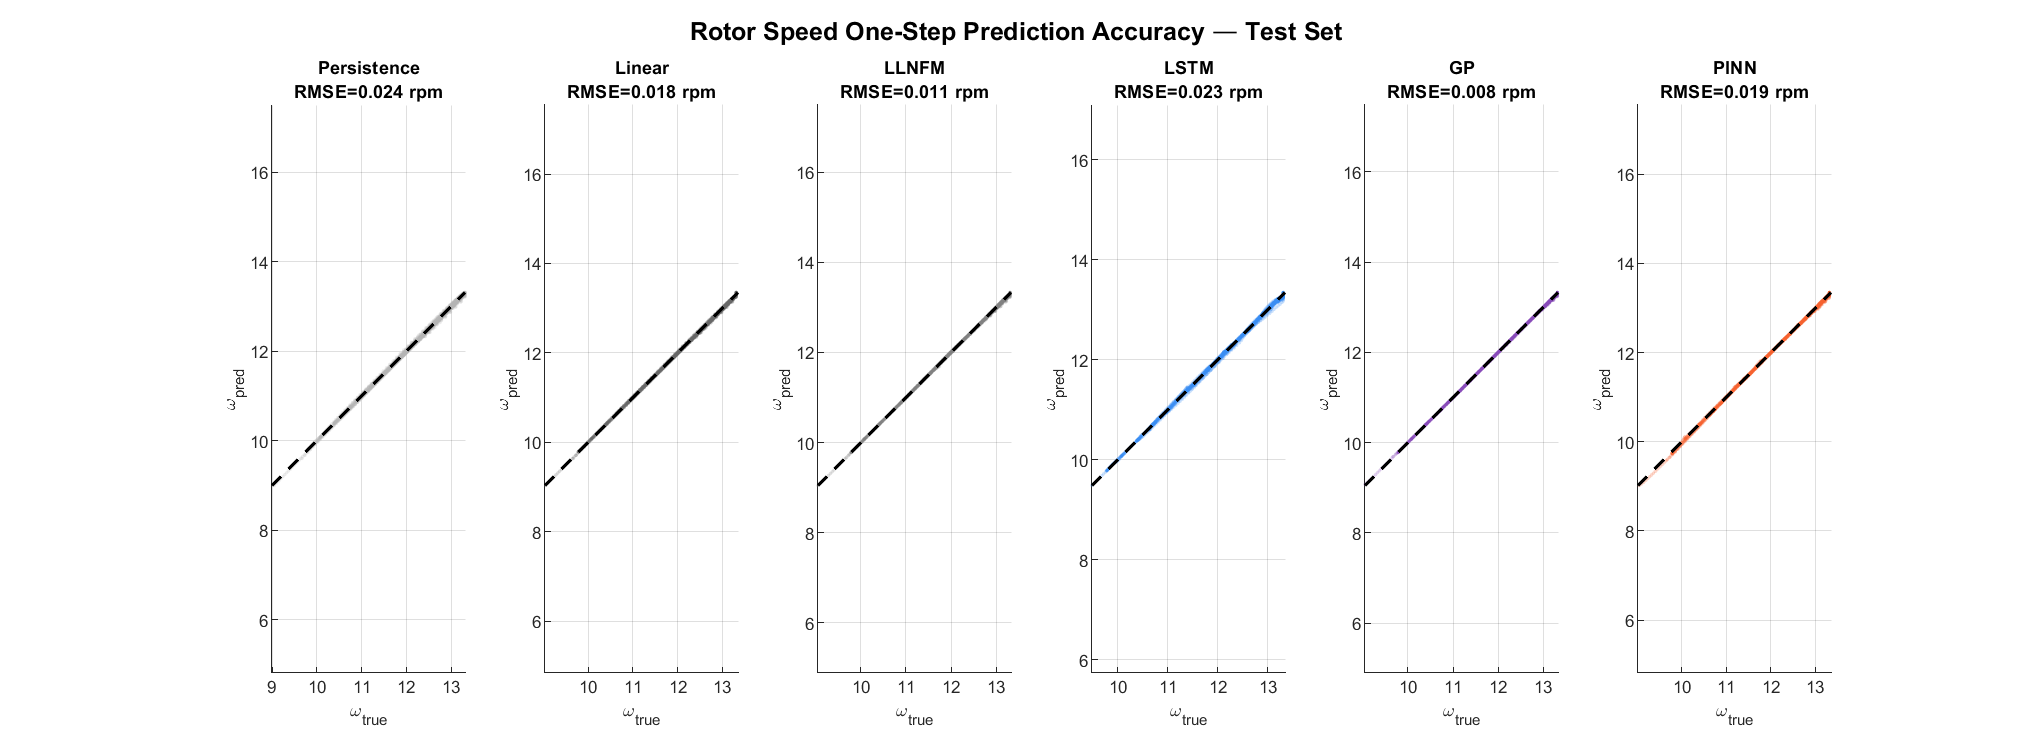
\includegraphics[width=0.85\textwidth]{figures/Fig2_S2_PredictionAccuracy.png}
\caption{Comparative test-set RMSE across all surrogate models, V1 and V2.}
\label{fig:stage2_rmse_bar}
\end{figure}
